\label{chap:introduction}

One of the main principles where \emph{Population Health Management (PHM)} and \emph{Clinical Decision Support (CDS)} are built upon is to improve the quality of healthcare for individuals and populations while reducing the operational healthcare overall costs. This raises the fundamental questions about \emph{how can healthcare quality be defined}?

One definition, by the Institute Of Medicine (IOM)\cite{iom2000} defines quality of care as the "the degree to which health services for individuals and populations increase the likelihood desired health outcomes and are consistent with the current professional knowledge". Tha means that to achieve the desired outcomes the underlying factors that contribute to the inconsistency of health outcomes need to be diminished. That is, the diagnostic errors themselves are handled and treated along the patient journey inside the healthcare providers.

\section{Medical Guidelines}

A medical guideline is a general practice that has been proven by gathered evidence and are considered a standard way of practicing medicine for specific clinical condition and outcomes. Several institutions are responsible for the definition and maintenance of these general practices. 

Such practices constitute a standard way of comparison between different institutions, practitioners and specially as a support to clinical decision over multidisciplinary complex situations. One good example of such complex clinical decision path is \emph{oncology}.

Some sample institutions that are regular producers of such evidence based general common practices are the National Comprehensive Cancer Network (NCCN)\cite{nccn2019}, The Fleischner Society Guideline (Fleischner 2017)\cite{fleischner2017}, The American College of Obstetricians and Gynecologists (ACOG)\cite{acog2019}.

These guidelines often also map how to reduce patient care risk and provide regarding appropriate rules to patient follow up. The patient follow up regarding their current condition status is important to avoid medical error and inappropriate diagnosis.

\section{Error in Medical Diagnosis}

IOM defines an error in medicine to be the “failure of a planned action to be completed as intended (i.e., error of execution) and/or the utilization of a wrong plan to achieve an aim (i.e., error of planning)”\cite{iom2004}. This definition also contemplates possible omissions as a failure. One example of such omission is not attending to the necessary patient follow up. Examples of medical errors:

\begin{itemize}
\item A misdiagnosis of any sort. All diagnosis should be evidence based and adhere to adequate clinical guidelines and \emph{status quo}
\item A failure to perform indicated tests and follow up exams, be it either lab or imaging
\item Failure to appropriately act on the results of tests on a timely manner. In this sense, under or overtreating the patient given it's clinical condition is also a failure
\end{itemize}

It is important to note that this definition of diagnostic error extends beyond the typical emphasis on avoidance \emph{misdiagnosis}. Instead, the definition of diagnostic error also includes the elements of timeliness and cost.

\section{Delivering Precision Medicine}

\begin{figure}
\begin{centering}
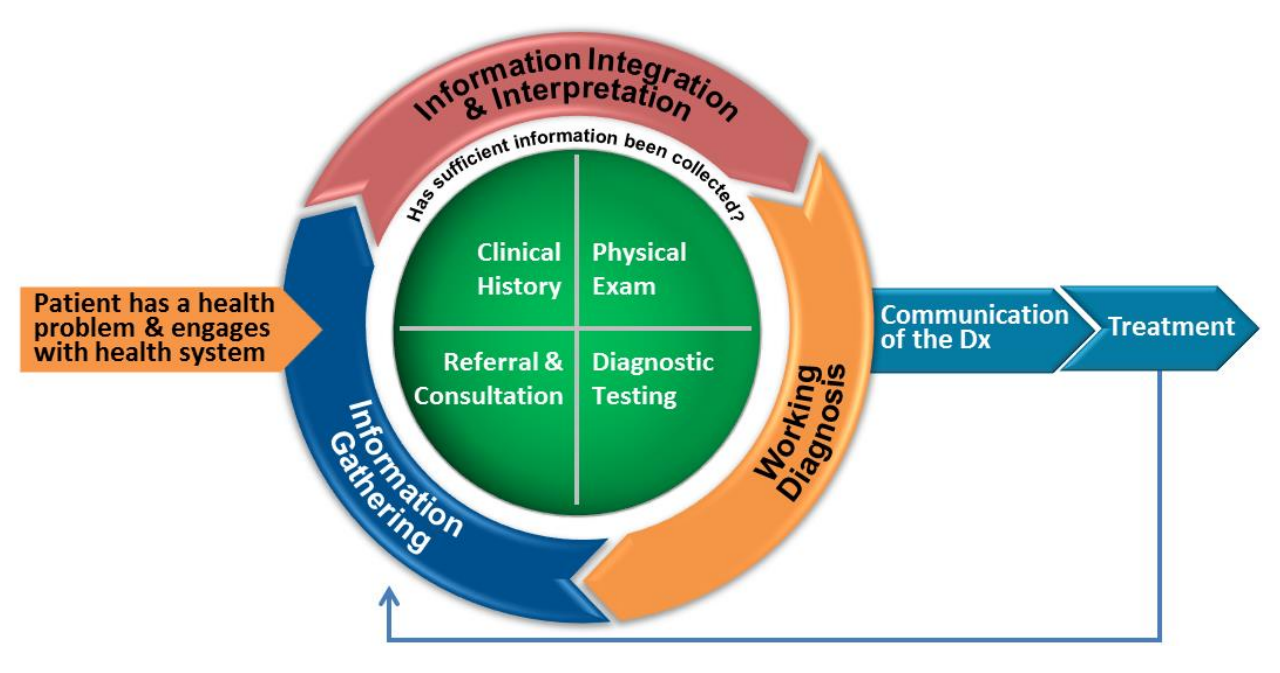
\includegraphics[width=1.0\textwidth]{DiagnosticProcess}
\par\end{centering}
\caption{\label{fig:DiagnosticProcess}The clinical diagnosis workflow along with the flow and gathering of the necessary information to support the clinical decision\cite{parasuraman2000}.}
%\vspace*{-44pt}
\end{figure}

The diagnostic process is a complex, collaborative activity that involves the synthesis of a patient’s clinical information from various sources, the goal of which is to identify the patient’s health problem. As such, this is a cyclic process consisting of acquiring, integrating, and interpreting which is the formation of a working diagnosis. 

As depicted by figure \ref{fig:DiagnosticProcess}, the process specifically includes the acquisition of the patient’s clinical history, performing hands-on physical examinations, diagnostic testing. The process of diagnostic testing is comprised of both medical imaging and laboratory analysis as well as consultation with other clinicians to seek additional expertise.

\begin{figure}
\begin{centering}
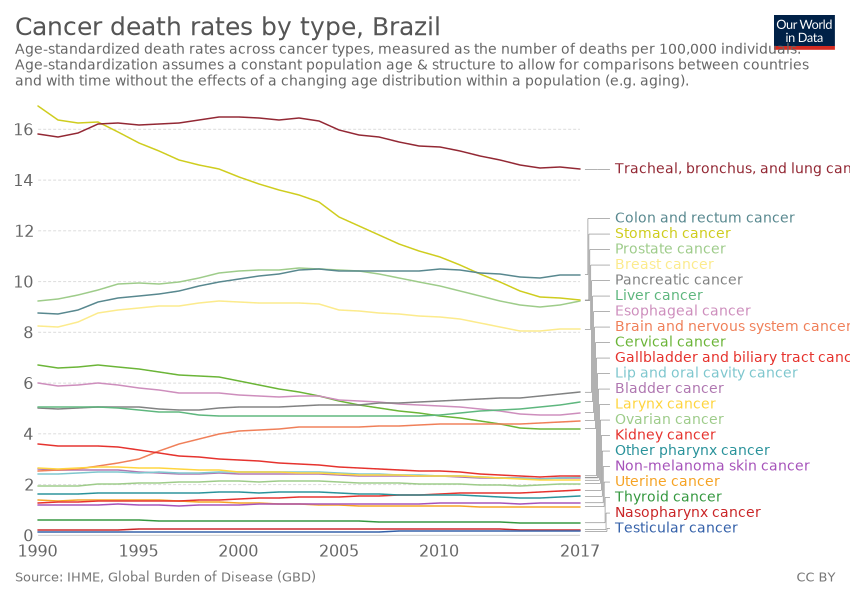
\includegraphics[width=1.0\textwidth]{CancerDeathRatesByTypeInBrazil}
\par\end{centering}
\caption{\label{fig:cancer_deaths_in_brazil}Cancer relative deaths by type in Brazil from 1990 to 2017.}
%\vspace*{-44pt}

\end{figure}

\section{Lung Cancer Screening}

Lung Cancer is of particular interest as the two most important factors for it is the patient tabagism history and age\cite{fleischner2017}. Also, the clinical workflow for it is very well defined and all incidental and malign nodules are identified and described by radiology reports, so adequate follow up is a matter of stakeholder communication between the different patient care providers to ensure that the patient does not falls into the gaps in medical care. 

For lung cancer screening the parameters of interest are the patient age, exposure to chemicals, the family oncology history and the patient tobacco smoking history\cite{fleischner2017, parasuraman2000, jaklitsch2012}.

Lung cancer is of particular interest due to it's high mortality ratio when compared with other cancers that could have even higher incidence. This trend can be seen in figure \ref{fig:cancer_deaths_in_brazil} and worse it is a trend that has been having a good resistance support which means that overall mortality for this type of cancer is hardly falling throughout the years.

\section{General Objective}

Extract a patient population for incidental lung nodule screening according to the available patient information in the \emph{Electronic Health Record (EHR)} and the \emph{Radiology Information System (RIS)} of the medical institution. 

\section{Specific Objectives}

The following are the guiding questions of interest for this work:

\begin{itemize}
  \item Identify each of the patient's variable of interest according to the NCCN and Fleischner 2017
  \item Map the different data silos in a medical institution where the guideline related informations could be obtained from
  \item Find out patients that are eligible for a follow up according to the available information in the Radiology Information System (RIS)
  \item Predict the patient risk profile according to it's own available health information
\end{itemize}

\section{Document Organization}

This document is organized in chapters with different goals. Chapter number \ref{chap:introduction} is introduces the general work thematic as well as a lung cancer screening overview; chapter \ref{chap:literature_review} performs a literature review of the state of art; number \ref{chap:methodology} talks about the data extraction methodology and results; and finally chapter \ref{chap:conclusion} is a review of the whole process along with a discussion of possibilities for improvements and future works.
